\chapter{Appendix: development and testing of knowledge based scoring functions for RosettaLigand initial placement}
\label{chap:lowres_appendix}
\section{Methods}

\subsection{Shape complementarity scoring grid}

\subsubsection{The need for and challenge of shape complementarity calculation}

Shape complementarity is a useful means of determining whether a ligand is in a well packed, non-clashing conformation relative to the protein binding pocket. 
However, rigorous computation of shape complementarity using a metric like $S_{c}$\citep{Lawrence:1993in}  is too time consuming for our purposes, so a rapid approximation of shape complementarity was developed.

\subsubsection{Description of shape complementarity calculations}

The shape complementarity scoring grid is computed by computing the distance between each square in the grid and the edge of the nearest protein atom, using the standard atom radii included in Rosetta.
The fully populated grid then represents the maximum possible radius that an atom at any given point within the grid can have without resulting in a clash with any other atom.
The effective complementarity of a given ligand atom is then computed by subtracting the radius of that atom from the value in the nearest grid square, resulting in the gap between the ligand atom and the nearest protein atom (Figure \ref{fig:shape_schematic}A). 
To compute an energy based on this gap, a knowledge based potential was used. 
The knowledge based potential was derived by computing the $-log(propensity)$ of a pair of protein and ligand atoms having a gap of a given distance length.
The knowledge based potential was derived using the Top8000 set of high quality crystal structures curated by the Richardson Lab.
The resulting potential is shown in Figure \ref{fig:shape_schematic}C.
The left hand (clashing) side of the potential is computed as a linear slope (indicated in red) when it passes above zero on the x axis, while the left hand side is computed as zero when it reaches the zero axis.
Atoms with large gaps are given scores of zero to avoid unnecessarily penalizing correct poses when a large portion of the ligand is exposed to solvent.
As RosettaLigand uses an implicit solvation model, solvent molecules are not present, and thus not represented in the scoring grid.
\begin{figure}
%figure 1 in original paper
\centering
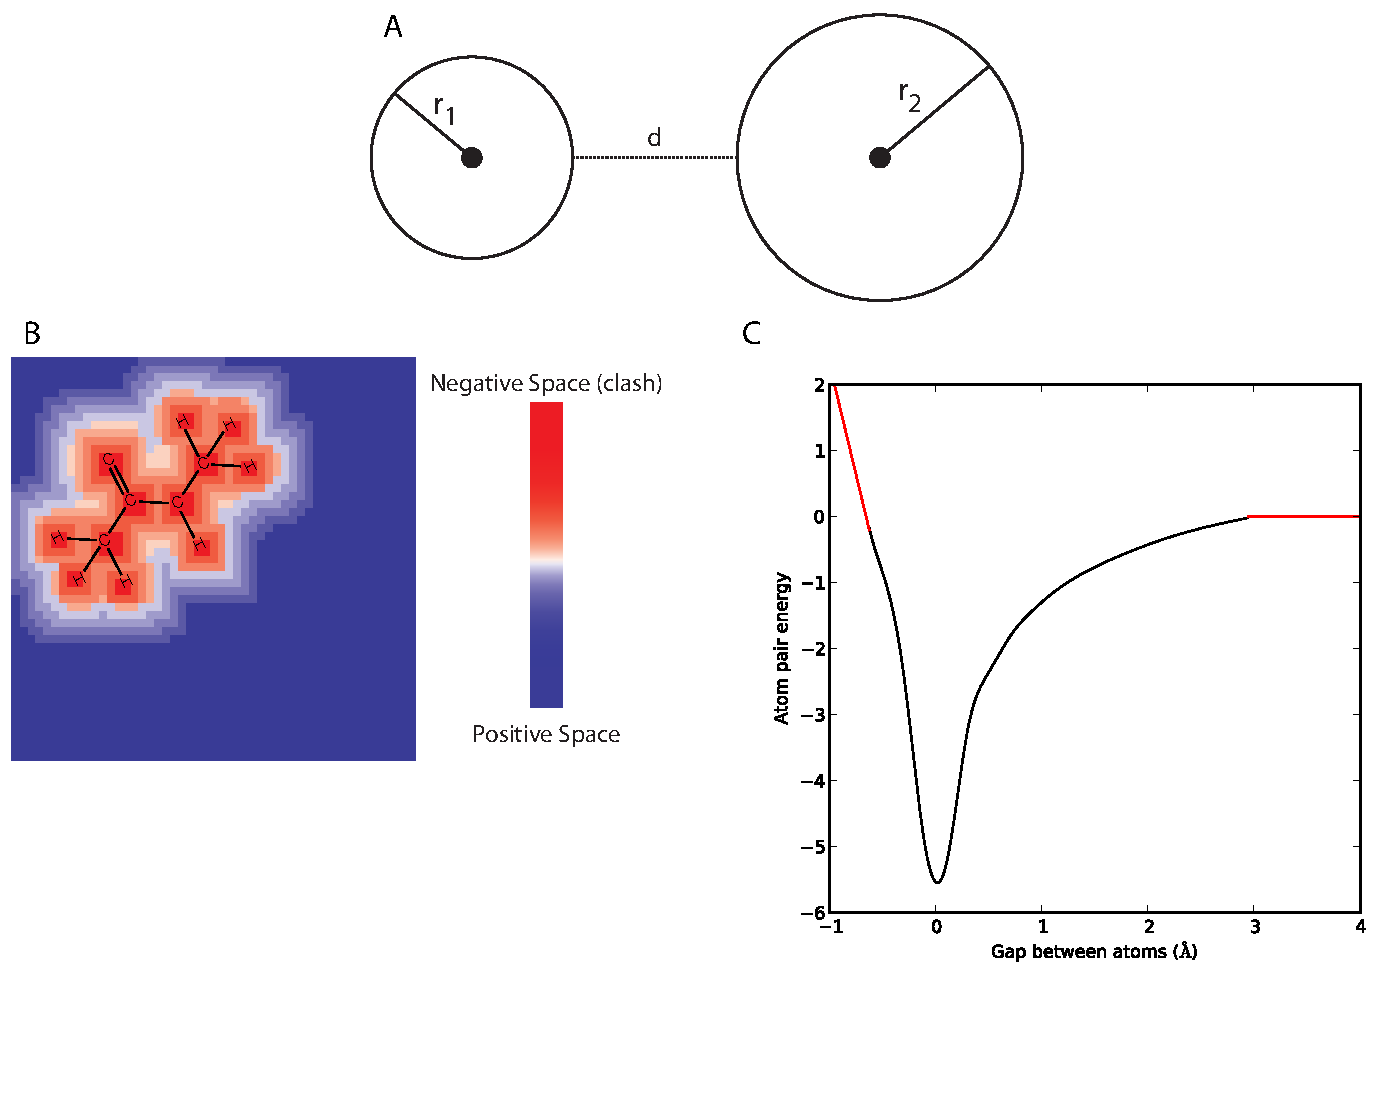
\includegraphics[width=6in]{figures/lowres_appendix/Shape_Complementarity.pdf}
\caption{
A schematic of the Shape Complementarity grid.
A) illustrates the computation of the gap distance between two atoms.
B) Represents the gap distances placed in the scoring grid.
C) Is a plot of the knowledge based potential.
In black is the region directly computed based on the knowledge based potential.
In red are linear functions applied to values beyond the bounds of the potential.
}
\label{fig:shape_schematic}
\end{figure}

\subsection{Hydrogen bond scoring grid}

\subsubsection{Description of hydrogen bond scoring calculations}

Two scoring grids are used to model hydrogen bonding.
As the goal of the initial placement algorithm is to provide a rapid first approximation of ligand position, only distance between hydrogen bond donor and acceptor are taken into account, and angular information is ignored.
A knowledge based potential was created based on the $-log(propensity)$ of a hydrogen bond donor atom being within some distance of a hydrogen bond acceptor atom, using the same Top8000 set of proteins described above (Figure \ref{fig:hbond_schematic}A).
Separate scoring grids are computed for hydrogen bond donors and acceptors. To compute the hydrogen bond donor scoring grid, the distance from each grid square to the nearest hydrogen bond donor is computed, and the score from the knowledge based potential is stored in the grid square (Figure \ref{fig:hbond_schematic}B).
The same process is followed to compute the hydrogen bond acceptor scoring grid.
Hydrogen bond donor atoms are scored based on the value of the nearest grid square in the appropriate scoring grid.  
The combination of the shape complementarity and hydrogen bonding scoring grids are referred to here as the "\ac{KBP}" scoring function. 
\begin{figure}
%figure 2 in original paper
\centering
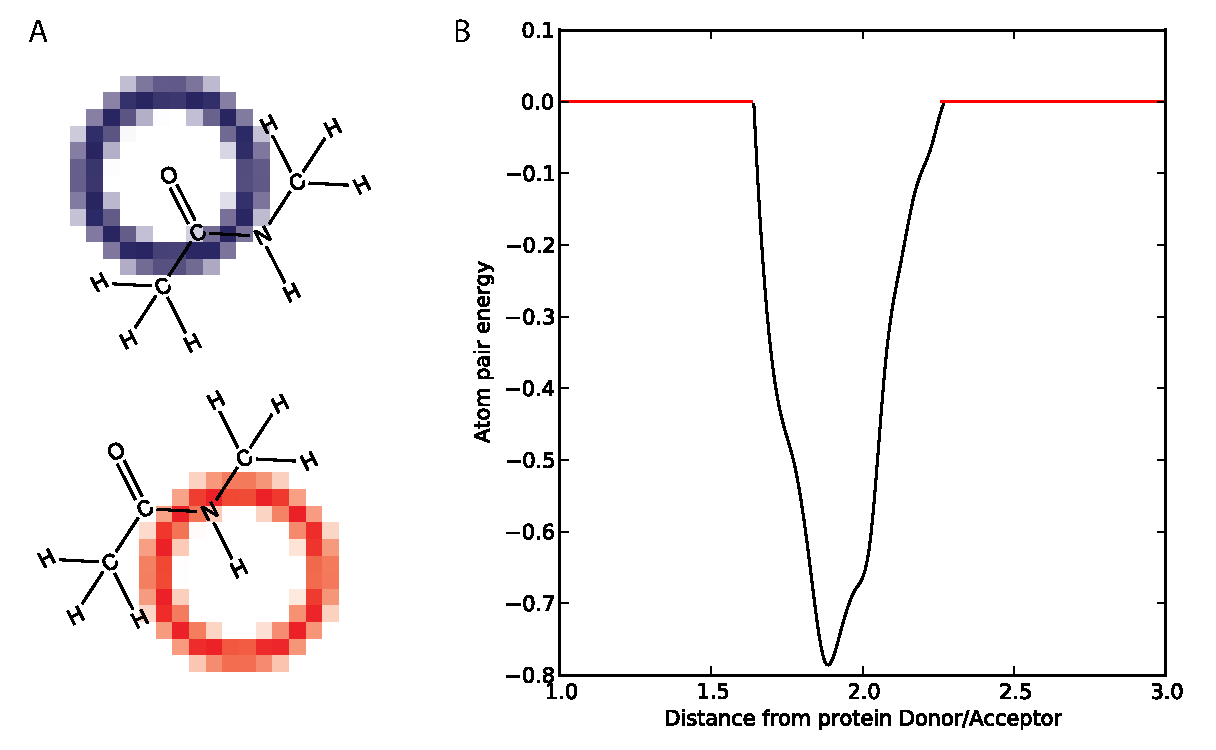
\includegraphics[width=6in]{figures/lowres_appendix/Hydrogen_Bonding.pdf}
\caption{
A schematic of the Hydrogen Bonding grid.
A) a schematic illustrating the placement of scoring information in the hydrogen bonding scoring grids.
B) the knowledge based potential used to populate the scoring grids.
In black is the region directly computed based on the knowledge based potential.  In red are linear functions applied to values beyond the bounds of the potential.
}
\label{fig:hbond_schematic}
\end{figure}

\section{Results and Discussion}

\subsection{The addition of the knowledge based shape complementarity and hydrogen bonding potentials does not improve sampling efficiency}

Figure \ref{fig:frac_time} and Figure \ref{fig:frac_count} compare the effect of the knowledge based potential on docking performance and efficiency.
Figure \ref{fig:frac_time}A and Figure \ref{fig:frac_count}A demonstrate that the new knowledge based potential no significant impact on ligand docking when docking into relaxed models.
Furthermore, when ligands are docked into repacked and relaxed models, the new Knowledge Based Potential demonstrates decreased performance compared to the binary scoring function. 
There are two factors which likely play a role in this decreased performance.
It is notable that as the degree of noise introduced into the protein structure increases, the performance of the \ac{KBP} based scoring grid relative to the Binary scoring grid decreases.
This is effect is most likely caused by the presence of side chain information in the \ac{KBP} based scoring grids.
Because side chain atoms are included, an input model with incorrect side-chains will result in an incorrectly placed energy minimum, and lower quality binding poses. 
The second likely factor is suggested by the shapes of the curves in Figure \ref{fig:frac_count}.
While most ligands are successfully docked within 150 poses, some ligands are exceptionally difficult to dock, and require additional sampling, for this reason, the Transform/Binary/Repack protocol shows a slight increase in success rate after approximately 800 models have been generated.
In contrast, the Transform/\ac{KBP}/Repack protocol does not exhibit the same increase.
This is likely a result of the comparative shapes of the two energy functions.
The Binary energy function is extremely flat, and results in a relatively wide area of space with identical scores.
As a result, a range of ligand poses will be produced during the initial placement stage, as there is not one single energy minimum.
On the other hand, the introduction of a knowledge based potential results in a scoring grid with one or more well defined energy minimums, which will reduce the diversity of allowed initial placements.
If these minima are incorrectly placed as a result of backbone inaccuracies, these incorrect minima will be extensively sampled, reducing overall accuracy of the docking process. 

\begin{figure}
%figure 3 in original paper
\centering
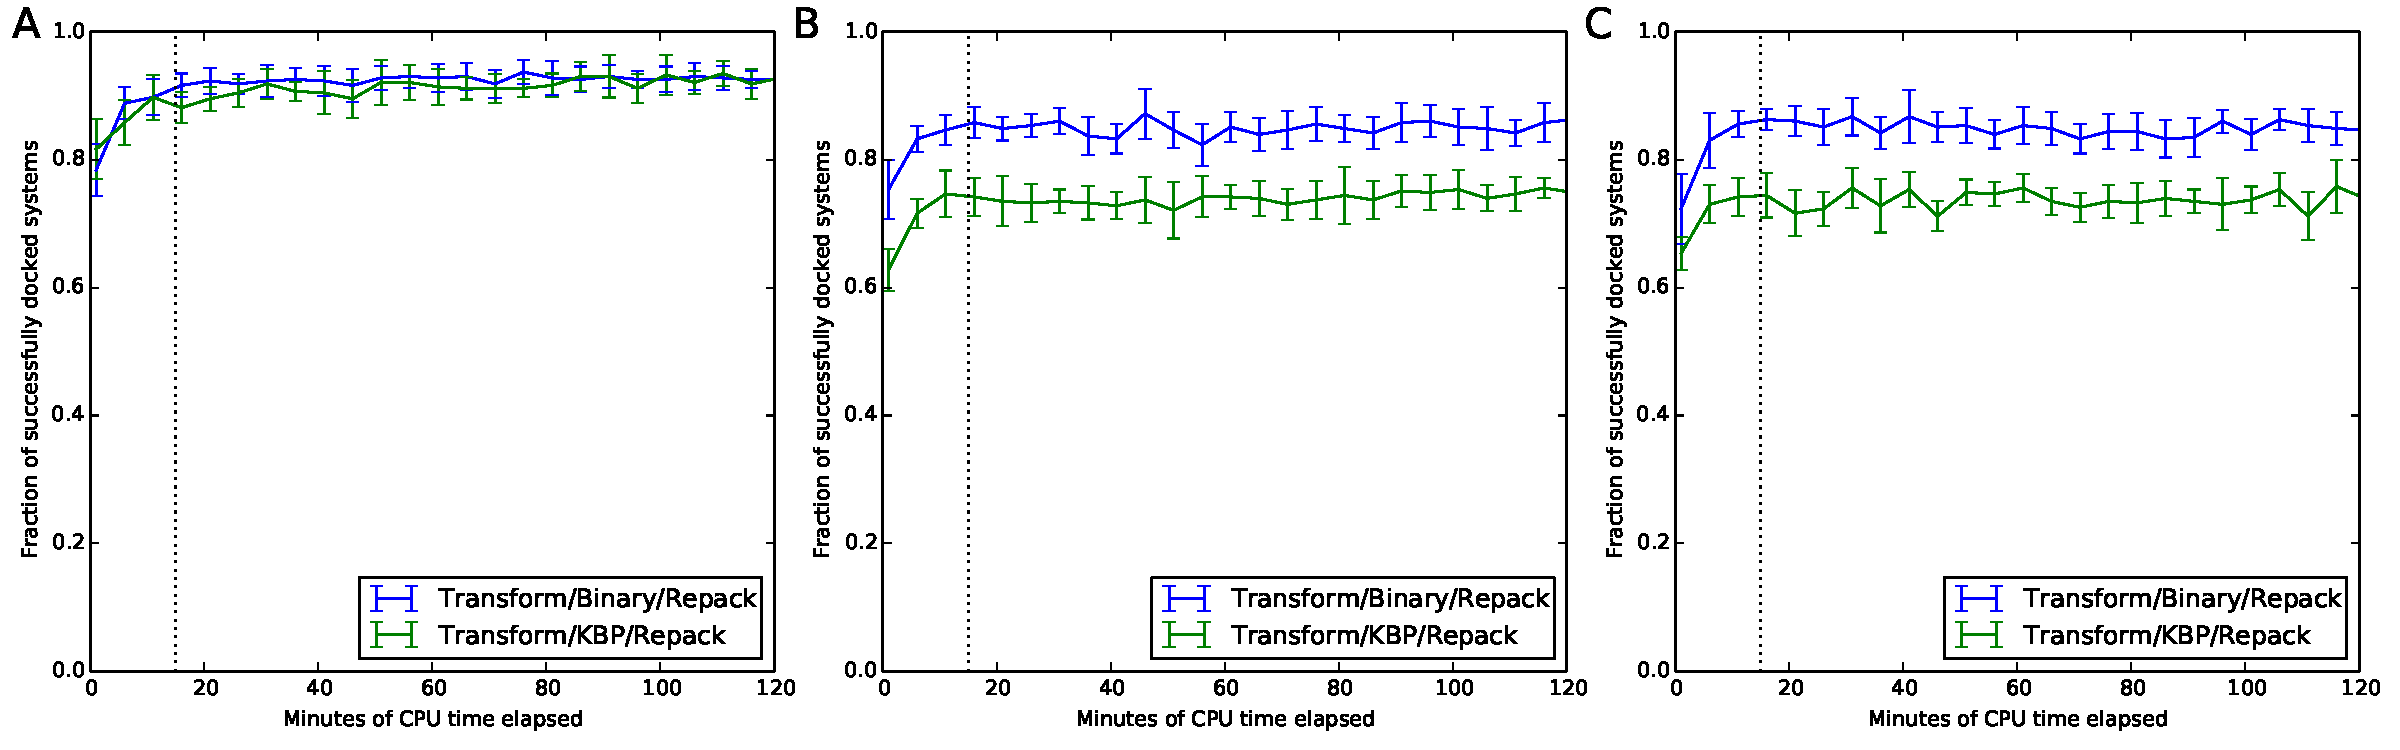
\includegraphics[width=6in]{figures/lowres_appendix/fraction_successful_time_supplement.pdf}
\caption{
The fraction of protein systems in which the lowest scoring model has an \acs{RMSD} < 2.0 \AA\ to the native structure as a function of \acs{CPU} time using the Binary scoring function (Transform/Binary/Repack) and Knowledge based scoring function (Transform/\acs{KBP}/Repack) RosettaLigand docking protocols when docked into A) Crystal structures, B) Repacked crystal structures and C) Relaxed crystal structures. 
A large pool of models were generated, and random subsamples were taken corresponding to time points at 5 minute intervals.
The number of structures included in each time point was based on the average time to generate a model for each algorithm.
20 random samples were taken for each time point, and the means are plotted, with the error bars representing the standard deviation. Docking protocols which make use of the Transform algorithm are reliably converged after approximately 15 minutes (dotted line).  
}
\label{fig:frac_time}
\end{figure}

\begin{figure}
%figure 4 in original paper
\centering
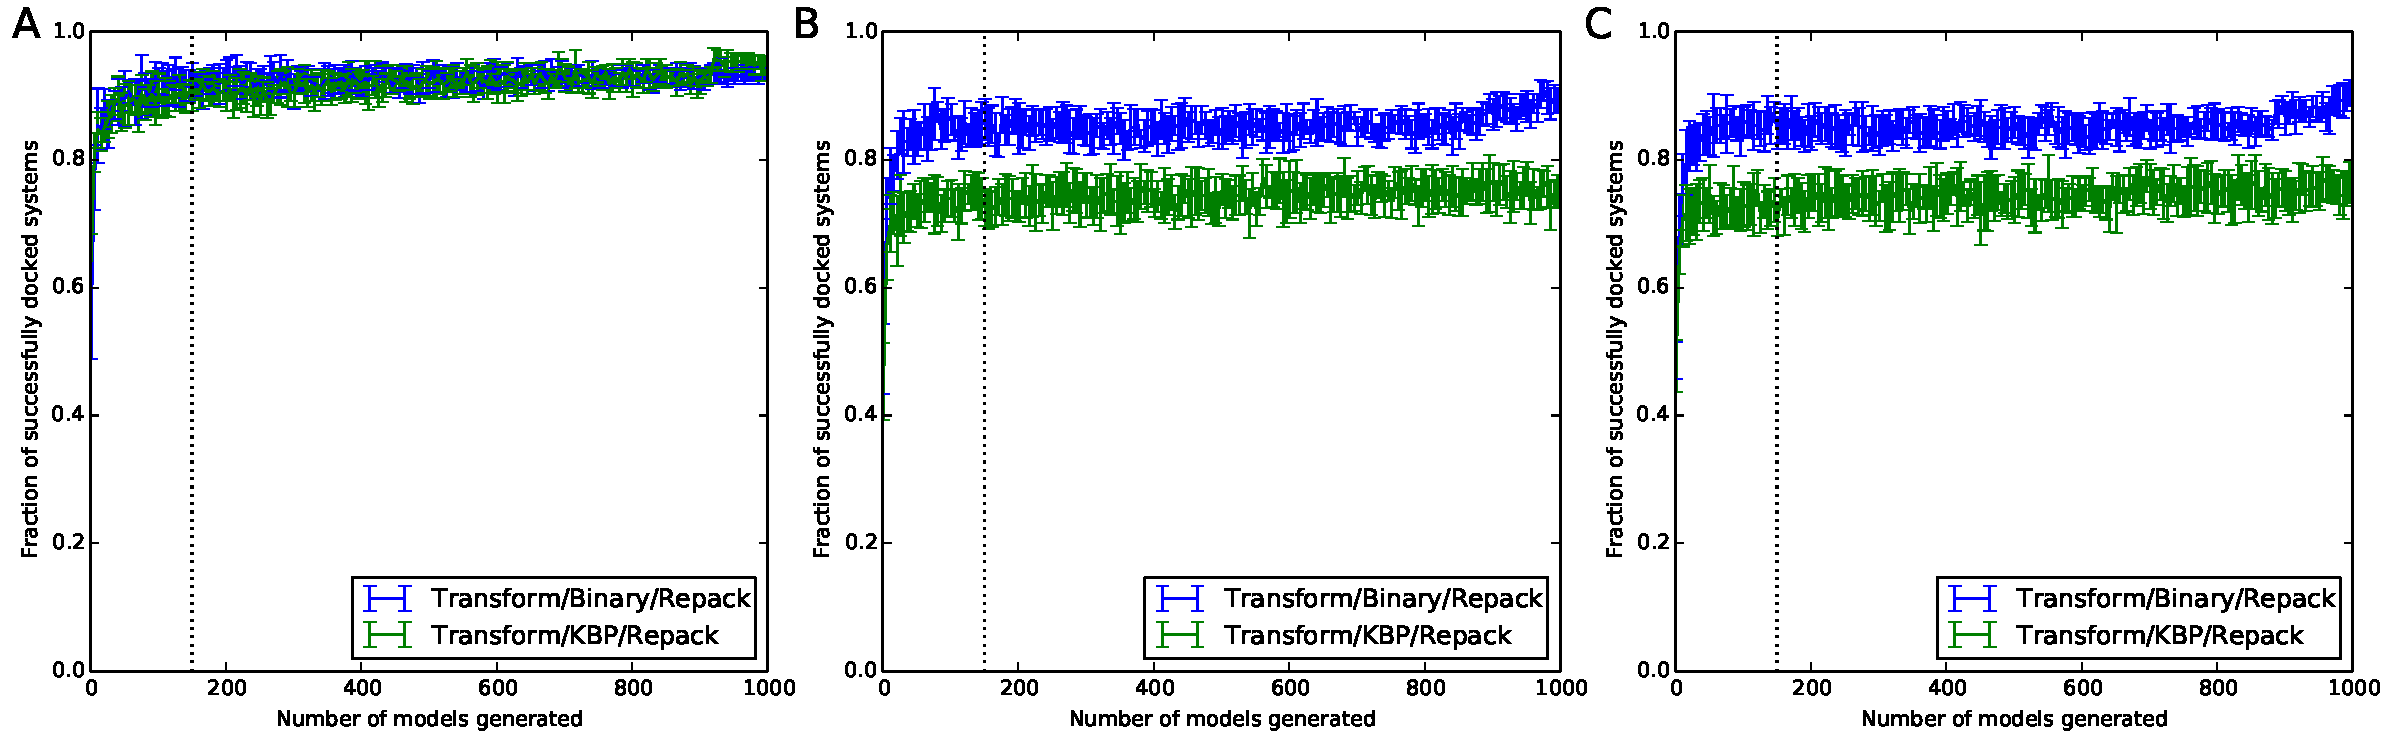
\includegraphics[width=6in]{figures/lowres_appendix/fraction_successful_count_supplement.pdf}
\caption{
The fraction of protein systems in which the lowest scoring model has an \acs{RMSD} < 2.0 \AA\ to the native structure as function of the total number of structures using the Binary scoring function (Transform/Binary/Repack) and Knowledge based scoring function (Transform/\acs{KBP}/Repack) RosettaLigand docking protocols when docked into A) Crystal structures, B) Repacked crystal structures and C) Relaxed crystal structures.
A large pool of models were generated, and random subsamples were taken.
20 random samples were taken for each point, and the means are plotted, with the error bars representing the standard deviation.
Docking protocols which make use of the Transform algorithm are reliably converged after approximately 150 models (dotted line).
}
\label{fig:frac_count}
\end{figure}

